\documentclass{article}
\usepackage{graphicx}
\graphicspath{ {images/} }
\usepackage[utf8]{inputenc}
\usepackage[czech]{babel}
\usepackage[
backend=biber,
style=numeric,
sorting=none
]{biblatex}
\usepackage[a4paper, total={6in, 8in}]{geometry}
\usepackage{subcaption}
\usepackage{amsmath}
\usepackage[utf8]{inputenc}
\usepackage{gensymb}

\title{EM1 - příklad 43}
\author{Matěj Vondráček \\ FJFI ČVUT}

\begin{document}

\maketitle

K výpočtům se bude hodit znát různé délky v šestiúhelníku. Označme $a$ jako jeho stranu a $b$ a $h$ jako odvěsny ve vyznačeném trojúhelníku. 

\begin{figure}[h]    
    \begin{subfigure}[b]{0.7\textwidth}
        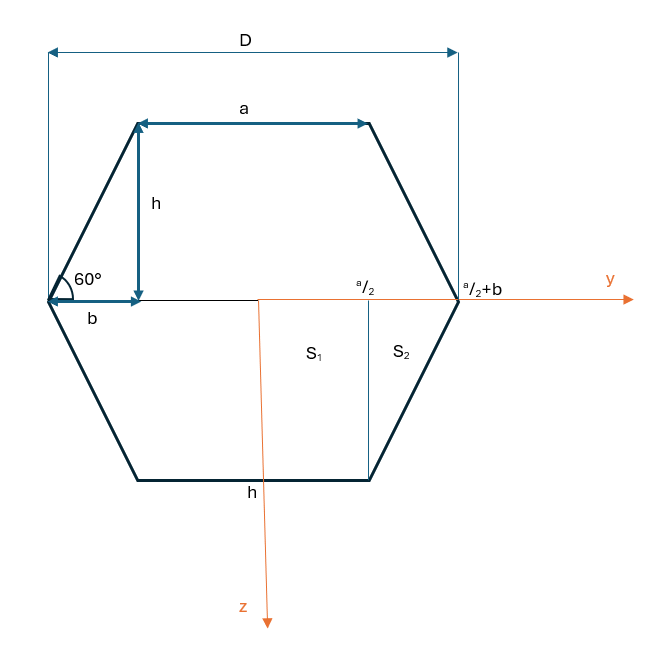
\includegraphics[width=\textwidth]{pic.png}
    \end{subfigure}
\end{figure}

Ze vztahů $D=a+2b$ a $\cos{60\degree}=\frac{b}{a}=\frac{1}{2}$ odvodíme $a=\frac{D}{2}$ a $b=\frac{a}{2} = \frac{D}{4}$.

Ze vztahu $\sin{60\degree}=\frac{h}{a}=\frac{\sqrt{3}}{2}$ pak odvodíme $h=\frac{\sqrt{3}}{2}a = \frac{\sqrt{3}}{4} D$.

\bigskip

Pro hlavní centrální kvadratické momenty platí:

\[ J_y=\iint\limits_{S} z^2\mathrm{d}S \] 
\[ J_z=\iint\limits_{S} y^2\mathrm{d}S \] 

\section{Kvadratický moment $J_y$}
Díky symetrii vždy stačí spočítat jen jeden kvadrant a výsledek vynásobit 4. Budeme počítat nejdřív $J_y$, přičemž rozdělíme obsah na dva: obdélník $S_1$ a trojúhelník $S_2$.

\[ J_y=4\iint\limits_{S} z^2\mathrm{d}S = 4\iint\limits_{S_1} z^2\mathrm{d}S + 4\iint\limits_{S_2} z^2\mathrm{d}S\] 

Spočítáme nejdřív první integrál.

\[ \iint\limits_{S_1} z^2\mathrm{d}S = \int_{0}^{\frac{a}{2}} \int_{0}^{h} z^2 \mathrm{d}z \mathrm{d}y = 
\int_{0}^{\frac{a}{2}}\left[\frac{z^3}{3}\right]_0^{\frac{\sqrt{3}}{2}a} \mathrm{d}y = \frac{1}{3}\int_{0}^{\frac{a}{2}} \frac{3 \sqrt{3}}{8}a^3 \mathrm{d}y =\]
\[= \frac{1}{3} \left[ \frac{3 \sqrt{3}}{8}a^3 \right]_0^{\frac{a}{2}} = \frac{\sqrt{3}}{8}a^3 \frac{a}{2} = \frac{\sqrt{3}}{16}a^4\]

Ke spočítání druhého integrálu je dobré si uvědomit, že podle Steinerových vět posuvu, má na kvadratický moment vliv jen posun kolmý k ose momentu, 
tzn. že můžeme zjednodušit meze v integrálu a posun od osy $z$ zanedbat. Dále potřebujeme odvodit funkci, která by vyjadřovala sklon trojúhelníku:

\[ z(0)=h=\frac{\sqrt{3}}{2}a \] 
\[ z(b)=0 \]

Řešením této soustavy dostáváme
\[ z(y)=-\frac{\sqrt{3}}{2}\frac{y}{b}+\frac{\sqrt{3}}{2}a = -\frac{\sqrt{3}}{a}y+\frac{\sqrt{3}}{2}a\]

Nyní jen dosadíme do integrálu:

\[ \iint\limits_{S_2} z^2\mathrm{d}S = \int_{0}^{b}\int_{0}^{-\frac{\sqrt{3}}{a}y+\frac{\sqrt{3}}{2}a} z^2 \mathrm{d}z \mathrm{d}y = 
\int_{0}^{\frac{a}{2}} \left[ \frac{z^3}{3}\right]_0^{-\frac{\sqrt{3}}{a}y+\frac{\sqrt{3}}{2}a} \mathrm{d}y 
= \frac{1}{3} \int_{0}^{\frac{a}{2}} \left(-\frac{\sqrt{3}}{a}y+\frac{\sqrt{3}}{2}a\right)^3 \mathrm{d}y\]

Použijeme substituci:
\[ u = -\frac{\sqrt{3}}{a}y+\frac{\sqrt{3}}{2}a\]
\[ \mathrm{d}u = -\frac{\sqrt{3}}{a} \mathrm{d}y\]

Pro meze pak platí:
\[ -\frac{\sqrt{3}}{a} \cdot \frac{a}{2} + \frac{\sqrt{3}}{2}a = 0\]
\[ -\frac{\sqrt{3}}{a} \cdot 0 + \frac{\sqrt{3}}{2}a = \frac{\sqrt{3}}{2}a\]

Po substituci dostáváme:
\[ \iint\limits_{S_2} z^2\mathrm{d}S = \frac{1}{3} \int_{\frac{\sqrt{3}}{2}a}^{0} -\frac{2}{\sqrt{3}}u^3 \mathrm{d}u 
= -\frac{2}{3\sqrt{3}} \left[\frac{u^4}{4}\right]_{\frac{\sqrt{3}}{2}a}^{0} = \frac{1}{3\sqrt{3} \cdot 2}\left(\frac{\sqrt{3}}{2}a\right)^4=
\frac{3}{\sqrt{3}}\frac{a^4}{32} = \frac{\sqrt{3}}{32}a^4\]


Pro kvadratický momement $J_y$ tedy platí

\[ J_y= 4 \left( \frac{\sqrt{3}}{16}a^4 + \frac{\sqrt{3}}{32}a^4 \right) = \frac{5\sqrt{3}}{16}a^4 = \frac{5\sqrt{3}}{256}D^4\]

\section{Kvadratický moment $J_z$}
Nyní budeme počítat kvadratický moment $J_z$. K němu obdobně potřebujeme odvodit funkci $y(z)$.

\[ y(0)=\frac{a}{2}+b = a\] 
\[ y(h)=y\left(\frac{\sqrt{3}}{2}a\right)=\frac{a}{2}\]

Řešením této soustavy dostáváme
\[ y(z)=-\frac{1}{\sqrt{3}}z+a \]

Nyní dosadíme do integrálu:
\[ J_z=4\iint\limits_{S} y^2\mathrm{d}S = 4\int_{0}^{h} \int_{0}^{-\frac{1}{\sqrt{3}}z+a} y^2 \mathrm{d}y \mathrm{d}z
= 4\int_{0}^{\frac{\sqrt{3}}{2}a} \left[\frac{y^3}{3}\right]_0^{-\frac{1}{\sqrt{3}}z+a}\mathrm{d}z =\]
\[= \frac{4}{3} \int_{0}^{\frac{\sqrt{3}}{2}a} \left(-\frac{1}{\sqrt{3}}z+a\right)^3 \mathrm{d}z\]

Použijeme substituci: 

\[u=-\frac{1}{\sqrt{3}}z+a\]  
\[\mathrm{d}u=-\frac{1}{\sqrt{3}}\mathrm{d}z\]

Pro meze pak platí:

\[-\frac{1}{\sqrt{3}}\frac{\sqrt{3}}{2}a + a = \frac{a}{2}\]
\[-\frac{1}{\sqrt{3}}\cdot 0 + a = a\]

Po dosazení do integrálu dostáváme:
\[ J_z = \frac{4}{3} \int_{a}^{\frac{a}{2}} -\sqrt{3} u^3 \mathrm{d}u = -\frac{4 \sqrt{3}}{3} \left[\frac{u^4}{4}\right]_{a}^{\frac{a}{2}} 
= -\frac{\sqrt{3}}{3} \left(\frac{a^4}{16}-\frac{a^4}{4}\right) = \frac{15}{16} \frac{\sqrt{3}}{3} a^4 = \frac{5 \sqrt{3}}{16}a^4
= \frac{5 \sqrt{3}}{256}D^4\]



\end{document}
